

\begin{minipage}{0.68\linewidth}
\textbf{Partie A} La figure ci-contre
représente une calotte sphérique de centre $O$, de rayon $r$ et de
hauteur $h$. Le volume d'un tel solide est donné par la formule
suivante
${\cal V}=\frac{\pi h^2}{3}(3r-h)$
\begin{enumerate}
\item Si une calotte sphérique a pour rayon $r=15$~cm et pour hauteur
$h=20$~cm, quel est son volume ?
\item Si une calotte sphérique a pour hauteur $h=9$~cm et pour volume
${\cal V}=81\pi$~cm$^3$, quel est son rayon ?
\item Si une calotte sphérique a pour hauteur $h=10$~cm et pour rayon
$r=6$~cm, quel est le rayon $r_1$ du cercle de section ?
\end{enumerate}

\textbf{Partie B} Un aquarium a la forme
d'une sphère de 16~cm de rayon coupée par deux plans
parallèles. Ces plans sont situés respectivement à 12,8~cm et
9,6~cm du centre.
\begin{enumerate}
\item Calcule l'aire des disques de section en fonction de $\pi$.
\item Calcule le volume de l'aquarium. On donnera la valeur exacte
puis une valeur approchée au mm$^3$ près.
\end{enumerate}
\end{minipage}
\hfill
\begin{minipage}{0.28\linewidth}
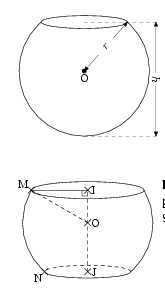
\includegraphics[scale=1]{RepS-43.png} 
\end{minipage}

